\subsection{Transformer}
\label{subsec:transformer}

\transformer{} adalah suatu jenis arsitektur jarigan yang baru dalam \dl{} yang digunakan untuk mentransformasi sebuah deretan data menjadi sesuatu dengan karakteristik, seperti panjang atau format, yang berbeda. Transformer tidak menggunakan lapisan rekursif (\rnn) atau konvolusi (\cnn).  Transformer menggunakan mekanisme \selfattention{} yang memungkinkannya untuk memahami hubungan antar elemen dalam sebuah deretan atau urutan
(\sequence). Tidak seperti pada \rnn{}, mekanisme \selfattention tidak perlu memperhatikan jarak antar elemen. Hal ini membuat \transformer{} menjadi sangat efisien untuk memproses data sekuensial. \transformer{} banyak digunakan pada proses penerjemahan bahasa, rangkuman teks, dan pengenalan suara.

\transformer{} terdiri atas dua komponen utama, yaitu \encoder{} dan \decoder. \encoderfl{} bertugas untuk membaca dan memproses sequence masukan, sementara \decoder{} menghasilkan \sequence{} keluaran berdasarkan informasi dari \encoder.

\encoderfl{} dan \decoder{} terdiri dari beberapa lapisan yang identik, dengan masing-masing memiliki dua sub-lapisan utama, yaitu:

\begin{enumerate}
	\item \mha~\\
	      Sublapisan ini menggunakan mekanisme \selfattention{} untuk memahami hubungan antar elemen dalam sebuah \sequence{}. Misalnya, dalam sebuah kalimat, mekanisme ini dapat mengenali bahwa kata "dia"
	      merujuk pada "ibu" meskipun terdapat kata-kata lain di antaranya.
	      \mha{} merupakan gabungan beberapa lapisan (\layer)
	      \emph{Scaled Dot-Product Attention} atau akan disingkat menjadi \attention. Perbandingan proses pada \mha{} dan \emph{Scaled Dot-Product Attention} dapat dilihat pada \autoref{fig:attention}

	      \begin{figure}[htbp]
		      \centering
		      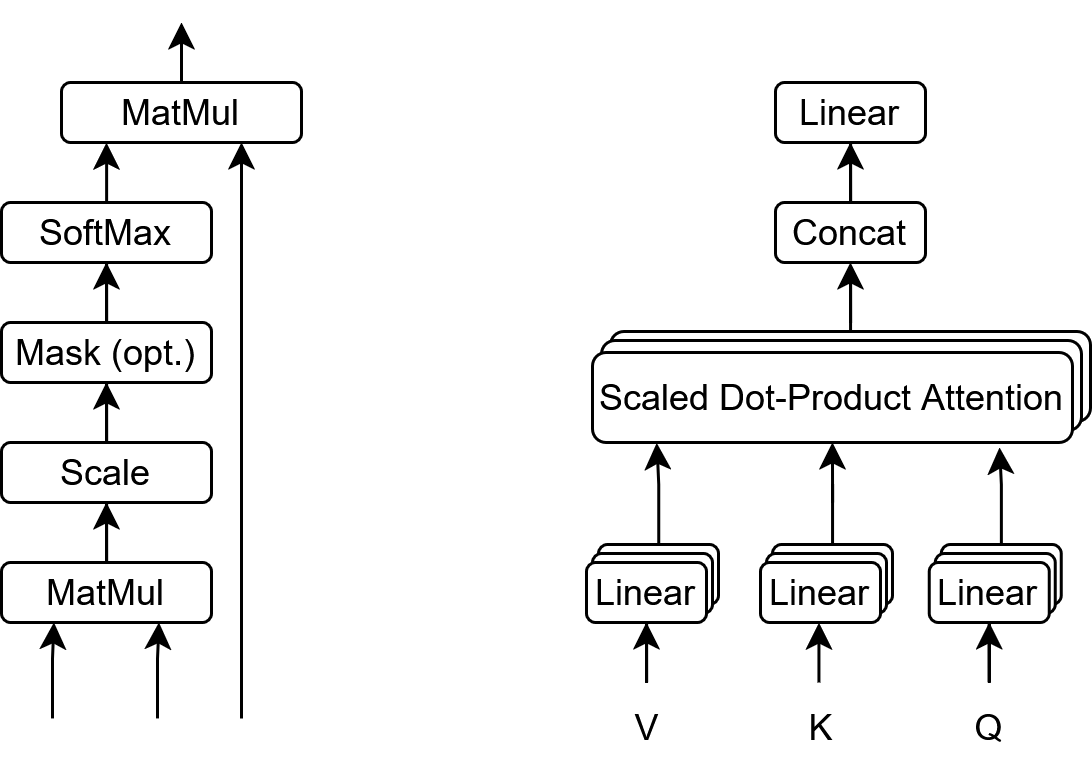
\includegraphics[width=.8\textwidth]{images/attentionmha.png}
		      \caption{\emph{Scaled Dot-Product Attention} (kiri) dan \mha{} (kanan) yang merupakan beberapa \layer{} \attention{} berjalan paralel \parencite{vaswani2017attention}}
		      \label{fig:attention}
	      \end{figure}

	      $Q$ (\emph{Query}), $K$ (\emph{Key}), dan $V$ (\emph{Value}) adalah representasi vektor dari setiap elemen dalam sebuah \sequence. Simbol $d_k$ adalah dimensi dari vektor $K$, yang digunakan untuk menskalakan hasil perkalian \emph{dot-product} $QK^\mathsf{T}$ agar proses pelatihan tetap stabil. Fungsi Softmax kemudian mengubah skor tersebut menjadi bobot probabilistik untuk menentukan elemen mana yang paling relevan untuk diperhatikan.

	      \pagebreak

	      Perhitungan \attention{} dilakukan dengan formula seperti yang ditunjukkan pada persamaan \eqref{eq:attention-softmax} \parencite{vaswani2017attention} yang didefinisikan sebagai berikut:

	      \begin{equation}
		      \label{eq:attention-softmax}
		      \operatorname{Attention}(Q, K, V) = \operatorname{SoftMax}\left(\frac{QK^\mathsf{T}}{\sqrt{d_k}}\right)V
	      \end{equation}
		  \addcontentsline{loe}{myequations}{\protect\numberline{\theequation}Persamaan Softmax}

	\item \ffnfull~\\
	      Setelah \attention{} dihitung, informasi dari setiap elemen diproses melalui jaringan \emph{feed-forward} yang sama untuk setiap posisi dalam urutan. Jaringan ini terdiri dari dua lapisan linear dengan fungsi aktivasi ReLU pada persamaan \eqref{eq:ffn} \parencite{vaswani2017attention}:

	      \begin{equation}
		      \label{eq:ffn}
		      \operatorname{FFN}(x) = \max(0, xW_1 + b_1)W_2 + b_2
	      \end{equation}
		  \addcontentsline{loe}{myequations}{\protect\numberline{\theequation}Fungsi Aktivasi ReLU pada \ffn}

	      \decoderfl{} memiliki perbedaan signifikan dibandingkan dengan \encoder.
	      \encoderfl{} terdiri dari beberapa lapisan yang masing-masing memiliki mekanisme \selfattention{} dan FFN. Setiap elemen dalam \sequence{} dapat saling “memperhatikan”. \decoderfl{} memiliki lapisan tambahan yang \encoder{}\--\decoder{} \attention. Lapisan ini memungkinkan \decoder{} untuk "memperhatikan" keluaran dari \encoder. \decoderfl{} memiliki mekanisme \emph{masking} untuk memastikan bahwa posisi saat ini hanya bergantung pada posisi sebelumnya.

	      \transformer{} memiliki keunggulan dibandingkan dengan metode konvensional pemrosesan sekuensial, yaitu \rnn. \transformer{} tidak bergantung
	      pada pemrosesan berurutan. \transformer{} dapat memproses seluruh urutan secara bersamaan, membuat pelatihan jauh lebih cepat. Implementasi \transformer{} menunjukkan hasil terbaik di berbagai kasus, seperti penerjemahan bahasa,
	      dibandingkan dengan arsitektur lainnya.

\end{enumerate}
